\documentclass[aspectratio=149]{beamer}
\usepackage[utf8]{inputenc}

\usepackage[utf8]{inputenc}
\usepackage[T1]{fontenc}

\usepackage[english]{babel}
\usepackage{amsmath}
\usepackage{cleveref}
\usepackage{amssymb}
\usepackage{mathtools}

%%Numbers, expectation
\newcommand{\N}{\mathbb{N}}
\newcommand{\E}{\mathbb{E}}
\renewcommand{\P}{\mathbb{P}}
\newcommand{\Var}{\mathbb{V}}
\newcommand{\R}{\mathbb{R}}
\newcommand{\D}{\mathcal{D}}
\newcommand{\B}{\mathcal{B}}
\newcommand{\Dh}{\D_h}
\renewcommand{\phi}{\varphi}
\newcommand*\diff{\mathop{}\!\mathrm{d}} % integral

%% mathoperator
\DeclareMathOperator*{\argmax}{arg\,max}
\DeclareMathOperator*{\argmin}{arg\,min}
\DeclareMathOperator*{\dom}{dom}
\DeclareMathOperator*{\sign}{sign}
\DeclareMathOperator*{\diag}{diag}

\DeclareMathOperator*{\Cov}{Cov}
\DeclareMathOperator*{\Cor}{Corr}
\DeclareMathOperator*{\Id}{Id}

%proximal operator
\newcommand{\prox}[3][]{\operatorname{prox}^{#1}_{#2}\left(#3 \right)}

\usepackage{xcolor}

%% sort citations by increasing number
\usepackage[sort,nocompress]{cite}

\usepackage{graphicx}% http://ctan.org/pkg/graphicx
\graphicspath{{../figures/}{../../figures}{../../memes}} %Setting the graphicspath
\usepackage{caption,subcaption}

\usepackage{tikz}
\usepackage{pgfplots}
\usetikzlibrary{backgrounds}
\usetikzlibrary{intersections}
\usepgfplotslibrary{fillbetween}

% \usepackage[right]{showlabels}


%%
\theoremstyle{plain}
\newtheorem{prop}{Proposition}[section]
\newtheorem{algo}{Algorithm}[section]
\newtheorem{assumption}{Assumption}
\theoremstyle{remark}
\newtheorem{remark}{Remark}[section]

% cref
\crefname{assumption}{Assumption}{Assumptions}
\crefname{equation}{}{}

\usepackage{autonum}

\usepackage{bm} %% bold math symbols

\usepackage{bbm} %% for \mathbbm{1}


% algorithmic environment
\usepackage{algorithm}
\usepackage[noend]{algpseudocode}

% for some reason this was required on one void linux installation (but not the other)
\usepackage{sansmathaccent}
\pdfmapfile{+sansmathaccent.map}

\author{Axel Böhm}

% shows which section we're in
\usetheme{Darmstadt}

% page number
\setbeamertemplate{footline}[frame number]
\setbeamercolor{page number in head/foot}{fg=gray}


% display things like onslide or visible already before but grayed out
\setbeamercovered{transparent}

% set the itemize item symbol as a diamond
\setbeamertemplate{itemize item}{$\diamond$}
% set the itemize subitem symbol as a triangle
\setbeamertemplate{itemize subitem}{$\blacktriangleright$}

% set the enumerate item symbol as a roman numbers
\setbeamertemplate{enumerate item}{(\roman{enumi})}


\author{Axel Böhm}

% shows which section we're in
\usetheme{Darmstadt}

% page number
\setbeamertemplate{footline}[frame number]
\setbeamercolor{page number in head/foot}{fg=gray}


% display things like onslide or visible already before but grayed out
\setbeamercovered{transparent}

% set the itemize item symbol as a diamond
\setbeamertemplate{itemize item}{$\diamond$}
% set the itemize subitem symbol as a triangle
\setbeamertemplate{itemize subitem}{$\blacktriangleright$}

% set the enumerate item symbol as a roman numbers
\setbeamertemplate{enumerate item}{(\roman{enumi})}


\title{Newton's and Quasi-Newton Methods}
\date{\today}


\begin{document}
\maketitle
\frame{\tableofcontents[]}

\section{Introduction}

\begin{frame}
  \frametitle{$1$-dimensional case: Newton-Raphson method}
  \textcolor{blue}{Objective:} Find zero of differentiable $f: \R \to \R$.
  \vspace{0.3cm}
  \begin{minipage}{0.48\textwidth}
    \textcolor{blue}{Strategy:} Solve
    \begin{equation}
      f(x_k) + f'(x_k) (x - x_k) = 0.
    \end{equation}
    \textcolor{blue}{Method:} Gives
    \begin{equation}
      x_{k+1} = x_k - \frac{f(x_k)}{f'(x_k)}
    \end{equation}
  \end{minipage}
  \hfill
  \begin{minipage}{0.48\textwidth}
    \begin{figure}[ht]
      \centering
      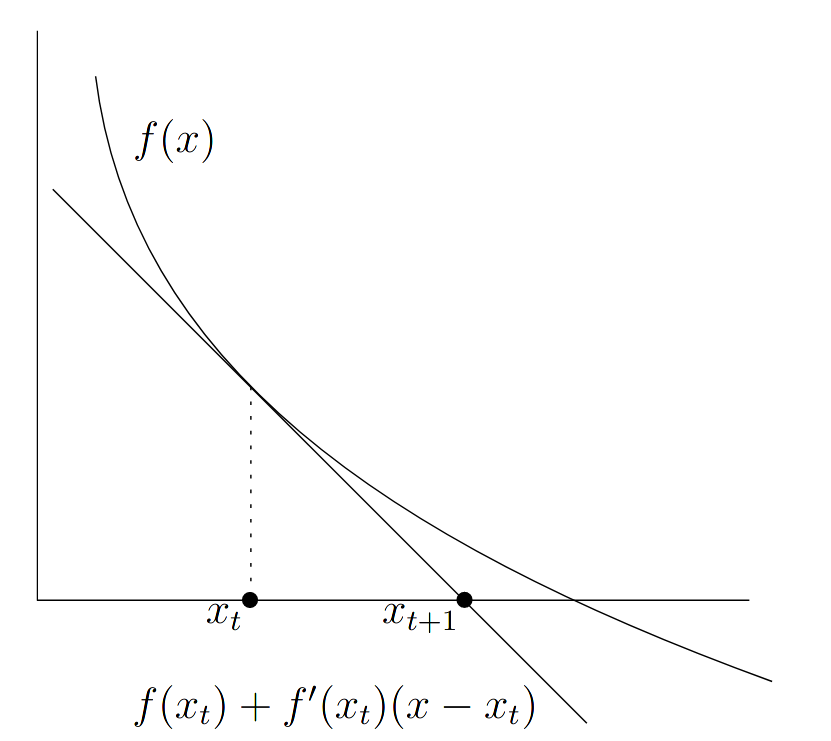
\includegraphics[width=\textwidth,height=\textheight,keepaspectratio]{newton-raphson}
      % \caption{\label{fig:label} }
    \end{figure}
  \end{minipage}
\end{frame}

\begin{frame}
  \frametitle{The Babylonian method}
  \begin{itemize}
    \item \textcolor{blue}{compute square root} of $R \in \R_+$
    \item find zero of $f(x) = x^2 - R$
    \item use Newton-Raphson:
          \begin{equation}
            x_{k+1} = x_k - \frac{f(x_k)}{f'(x_k)} = x_k - \frac{x_k^2 - R}{2 x_k} = \frac12 \left( x_k + \frac{R}{x_k} \right)
          \end{equation}
    \item Starting from $x_0 > 0$ we have
          \begin{equation}
            x_{k+1} = \frac12 \left( x_k + \frac{R}{x_k} \right) \ge \frac{x_k}{2}.
          \end{equation}
    \item Starting from $x_0 = R \ge 1$, it takes $\mathcal{O}(\log R)$ steps to get to $x_k - \sqrt{R} < \frac12$.
  \end{itemize}
\end{frame}

\begin{frame}
  \frametitle{The Babylonian method - Takeoff}
  \onslide<1>{%
    Note that
    \begin{equation}
      x_{k+1} - \sqrt{R} = \frac12 \left( x_k + \frac{R}{x_k} \right) - \sqrt{R} = \frac{x_k}{2} + \frac{R}{2 x_k} - \sqrt{R} = \frac{1}{2 x_k} {\left( x_k - \sqrt{R} \right)}^2
    \end{equation}
    For simplicity $R \ge 1/4$, then $x_k \ge \sqrt{R} \ge 1/2$. Hence
    \begin{equation}
      x_{k+1} - \sqrt{R} = \frac{1}{2 x_k} {\left( x_k - \sqrt{R} \right)}^2 \le {\left( x_k - \sqrt{R} \right)}^2
    \end{equation}
  }

  \onslide<2->{%
    If $x_0 - \sqrt{R} < \frac12$ (ensured after $\mathcal{O}(\log R)$ steps).
    \begin{equation}
      x_{k} - \sqrt{R} \le {\left( x_0 - \sqrt{R} \right)}^{2^k} \le {\left(\frac12\right)}^{2^k}
    \end{equation}
    To achieve $x_k - \sqrt{R} < \epsilon$ we only need $k = \log \log (\epsilon^{-1})$ steps!
  }
\end{frame}

\begin{frame}
  \frametitle{The Babylonian method - Example}
  $R=1000$, in double arithmetic
  \begin{itemize}
    \item $7$ steps to get to $x_7 - \sqrt{1000} < 1/2$
          \item $3$ steps to get to $\sqrt{1000}$ up to \textit{machine precision}
          \item First phase: $\approx$ \textcolor{blue}{one more correct digit} per iteration
          \item Second phase: $\approx$ \textcolor{blue}{double the number of correct digits} per iteration
  \end{itemize}

  \begin{center}
    In practice: $\log \log x \le 5$.
  \end{center}

\end{frame}


\section{Newton's method}%

\begin{frame}
  \frametitle{Newton's method for optimization}
  \begin{itemize}
    \item \textcolor{blue}{Goal:} Find global minimum $x^*$ of convex, differentiable function $f$.
    \item \textcolor{blue}{Strategy:} Search for zero of derivative.
    \item \textbf{$1$-dimensional case:} Apply Newton-Raphson method to $f'$:
          \begin{equation}
            x_{k+1} = x_k - \frac{f'(x_k)}{f''(x_k)} = x_k - {f''(x_k)}^{-1} f'(x_k)
          \end{equation}
          (requires \textcolor{blue}{twice} differentiable and $f'' > 0$)

    \item \textbf{$d$-dimensional case:} Newtons methods for minimizing convex $f: \R^d \to \R$:
          \begin{equation}
            x_{k+1} = x_k - {\nabla^2 f(x_k)}^{-1} \nabla f(x_k).
          \end{equation}
  \end{itemize}
\end{frame}


\begin{frame}
  \frametitle{Newton's method as adaptive gradient descent}
  General update scheme:
  \begin{equation}
    x_{k+1} = x_k - H(x_k) \nabla f(x_k)
  \end{equation}
  for some matrix $H(x) \in \R^{d \times d}$.
  \begin{itemize}
    \item \textcolor{blue}{Newton's method}: $H = {\nabla^2 f(x_k)}^{-1}$.
    \item \textcolor{blue}{Gradient descent}: $H = \alpha \Id$
  \end{itemize}
  \vspace{1cm}
 \begin{block}{}
  Newton's methods \textbf{adapts} to the local geometry of $f$ at $x_k$ \\
 \end{block}
  $\rightarrow$ \textit{no need to choose a stepsize}.
\end{frame}

\begin{frame}
  \frametitle{Convergence in one step on quadratic functions}
  A \textcolor{blue}{quadratic} function
  \begin{equation}
    f(x) = \frac12 x^T M x + q^T x + c
  \end{equation}
  is called \textit{nondegenerate} if $M$ is invertible.
  \begin{itemize}
    \item $x^* := M^{-1}q$ is the unique solution of $\nabla f(x) = 0$.
    \item $x^*$ is the unique global minimum if $f$ is convex.
  \end{itemize}
  \begin{lemma}[\textcolor{gray}{arbitrary $x_0$}]%
    On nondegenerate quadratic functions, Newtons method yields $x_1=x^*$.
  \end{lemma}
  \begin{proof}
    We have $\nabla f(x) = Mx -q$ and $\nabla^2 f(x) = M$. Therefore
    \begin{equation}
      x_1 = x_0 - {\nabla^2 f(x_0)}^{-1} \nabla f(x_0) = x_0 - M^{-1}(M x_0 - q) = M^{-1}q = x^*. \qed\qedhere
    \end{equation}
  \end{proof}
\end{frame}

% \begin{frame}
%   \frametitle{Affine Invariance}
%   Newton’s method is \textcolor{blue}{affine invariant}
%   (invariant under any invertible affine transformation):
%   Denote the Newton step for $h$ by
%   \begin{equation}
%     N_h(x) := x - {\nabla^2 h }^{-1} \nabla h(x).
%   \end{equation}
%   \begin{lemma}%
%     Let $f: \R^d \to \R$ be twice differentiable, $A \in \R^{d \times d}$ an invertible matrix and $b \in \R^d$.
%     \begin{equation}
%       g(x) = Ax + b.
%     \end{equation}
%     Then
%     \begin{equation}
%       N_{f \circ g} = g^{-1} \circ N_f \circ g
%     \end{equation}
%   \end{lemma}
% \end{frame}

% \begin{frame}
%   \frametitle{}
%   \begin{figure}[ht]
%     \centering
%     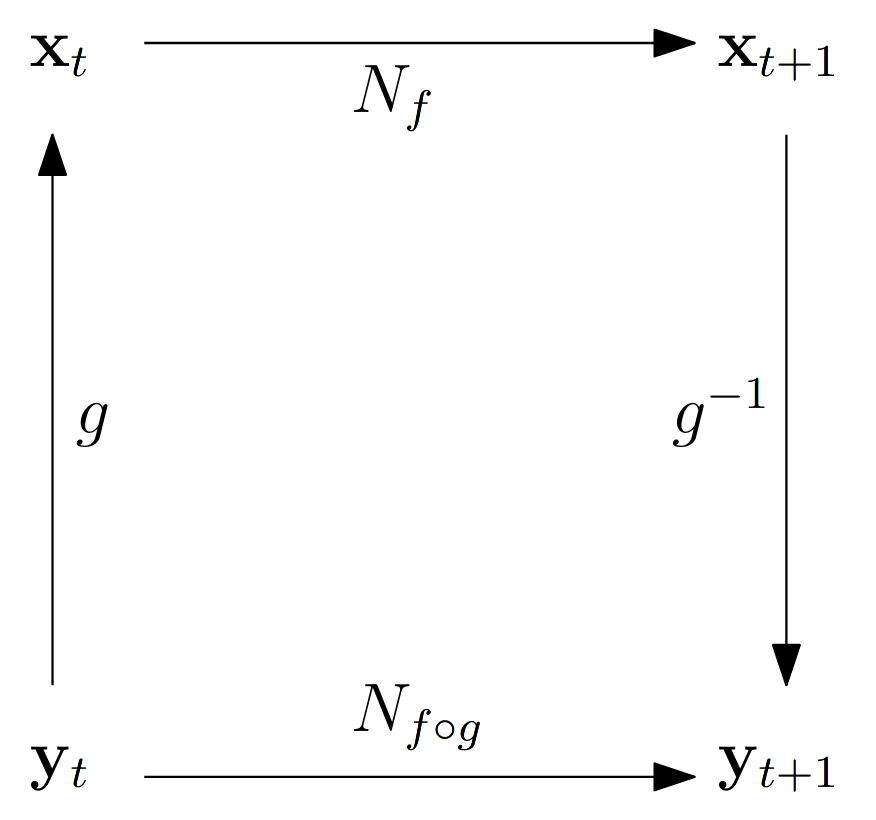
\includegraphics[width=\textwidth,height=\textheight,keepaspectratio]{newton_aff_invariance}
%     % \caption{\label{fig:label} }
%   \end{figure}
%   Gradient descent suffers if coordinates are at different scales; Newton's method doesn't.
% \end{frame}


\begin{frame}
  \frametitle{Minimizing the second-order Taylor approximation}
  Alternative interpretation of Newton's method:\\
  \begin{block}{}
    \center
    Minimize (local) \textcolor{blue}{quadratic model} of $f$.
  \end{block}
  \begin{lemma}%
    Let $f$ be convex, twice differentiable and $\nabla^2 f(x_k) \succ 0$. Then $x_{k+1}$ resulting from \textbf{Newton's step} satisfies
    \begin{equation}
      x_{k+1} = \argmin_{x \in \R^d} \left\{f(x_k) + \langle \nabla f(x_k), x-x_k \rangle + \frac12 \big \langle x-x_k, \nabla^2 f(x_k) (x-x_k)  \big\rangle \right\}
    \end{equation}
  \end{lemma}
\end{frame}


\begin{frame}
  \frametitle{Local Convergence}
  \textcolor{gray}{We will prove:}\\
  Under suitable conditions on $f$ and \textcolor{blue}{close to the minimum} Newton's method approximates solution up to an error $\epsilon$ in \textcolor{blue}{$\log \log (1/\epsilon)$} iterations.
  \begin{itemize}
    \item much faster than anything so far..
    \item only locally
  \end{itemize}
  \begin{block}{}
    We call this a \textcolor{blue}{local convergence} result.\\
  \end{block}

  \textcolor{blue}{Global convergence} statements are more difficult to obtain.
\end{frame}


\section{Convergence analysis}%

\begin{frame}
  % \frametitle{Theorem + Technical conditions }
  \begin{theorem}
    Let $f$ be convex with unique global minimum $x^*$, and $X$ a ball around $x^*$ s.t.
    \begin{enumerate}
      \item \textcolor{blue}{Bounded inverse Hessians:} There exists $\mu > 0$
            \begin{equation}
              \Vert {\nabla^2 f(x)}^{-1} \Vert \le \frac{1}{\mu}, \quad \forall x \in X
            \end{equation}
      \item \textcolor{blue}{Lipschitz continuous Hessians:} There exists $B>0$
            \begin{equation}
              \Vert \nabla^2 f(x) - \nabla^2 f(y) \Vert \le B \Vert x-y \Vert, \quad \forall x,y \in X
            \end{equation}
    \end{enumerate}
    Then, for $x_{k+1} = N_f(x_k)$ we have
    \begin{equation}
      \Vert x_{k+1} -x^* \Vert \le \frac{B}{2 \mu} \Vert x_k - x^* \Vert^2.
    \end{equation}
  \end{theorem}
\end{frame}


\begin{frame}
  \frametitle{Super-exponential speed}
  \begin{corollary}%
    In the setting of previous theorem, if
    \begin{equation}
      \Vert x_0 - x^* \Vert \le \frac{\mu}{B},
    \end{equation}
    then
    \begin{equation}
      \Vert x_k -x^*  \Vert \le \frac{\mu}{B} {\left( \frac{1}{2} \right)}^{2^k-1}
    \end{equation}
  \end{corollary}
  Close to the global minimum, we will reach distance to the minimum less than $\epsilon$ in at most $\log \log (1/\epsilon)$ steps.

  \textcolor{gray}{As for the last phase of Babylonian method.}
\end{frame}


\begin{frame}
  \frametitle{Super-exponential speed - intuition}

  \begin{itemize}
    \item Almost constant Hessians close to optimality...
    \item so $f$ behaves almost like a quadratic
    \item on which Newton's converge in one step
  \end{itemize}

  \begin{lemma}%
    If
    \begin{equation}
      \Vert x_0 - x^* \Vert \le \frac{\mu}{B}
    \end{equation}
    the Hessians in Newton's method satisfy the \textcolor{blue}{relative error bound}
    \begin{equation}
      \frac{\Vert  \nabla^2 f(x_k) - \nabla^2 f(x^*) \Vert}{\Vert \nabla^2 f(x^*) \Vert} \le {\left( \frac12 \right)}^{2^k-1}.
    \end{equation}
  \end{lemma}
\end{frame}


\begin{frame}
  \frametitle{Proof of convergence theorem}
  We abbreviate $H = \nabla^2 f(x_k)$, $x=x_k$, $x^+ = x_{k+1}$
  \begin{equation}
    \begin{aligned}
      x^+ - x^* &= x - x^* - H^{-1} \nabla f(x) \\
      &= x - x^* + H^{-1}( \nabla f(x^*) - \nabla f(x)) \\
      &= x - x^* + H^{-1} \int_{0}^{1} H(x + t(x^* - x))(x^* - x) \diff t,
    \end{aligned}
  \end{equation}
  \onslide<2->{%
    where we used the fundamental theorem of calculus
    \begin{equation}
      \int_{a}^{b} h' (t) \diff t
    \end{equation}
    with
    \begin{align}
      h(t)  &= \nabla f(x + t(x^* -x )) \\
      h'(t) &= \nabla^2f (x + t(x^* -x ))(x^*-x).
    \end{align}
  }
\end{frame}


\begin{frame}
  \frametitle{Proof of convergence theorem II}
  So far
  \begin{equation}
      x^+ - x^* = x - x^* + H^{-1} \int_{0}^{1} H(x + t(x^* - x))(x^* - x) \diff t
  \end{equation}
  With
  \begin{equation}
    x- x^* = {H(x)}^{-1} \int_{0}^{1} - H(x)(x^*-x)
  \end{equation}
  we get
  \begin{equation}
    x^+ - x^* =  H^{-1} \int_{0}^{1} (H(x + t(x^* - x))- H(x))(x^* - x) \diff t.
  \end{equation}
  Using norms
  \begin{equation}
    \Vert x^+ - x^*  \Vert \le  \Vert H^{-1} \Vert \left\Vert  \int_{0}^{1} H(x + t(x^* - x))- H(x)(x^* - x) \diff t \right\Vert
  \end{equation}
\end{frame}


\begin{frame}
  \frametitle{Proof of convergence theorem III}

  \begin{align}
    \Vert x^+ - x^*  \Vert &=  \Vert H^{-1} \Vert \left\Vert  \int_{0}^{1} (H(x + t(x^* - x))- H(x))(x^* - x) \diff t \right\Vert \\
    &\le \Vert H^{-1} \Vert  \Vert x^* - x \Vert \int_{0}^{1} \left\Vert  (H(x + t(x^* - x))- H(x)) \right\Vert \diff t
  \end{align}
  Use \textbf{bounded inverse Hessians} and \textbf{Lipschitz continuity} of the Hessian to conclude
  \begin{align}
    \Vert x^+ - x^*  \Vert  &\le \frac{1}{\mu} \Vert x^* - x \Vert \int_{0}^{1} B \Vert t(x^*-x) \Vert \diff t  \\
    &= \frac{B}{\mu} \Vert x^*-x \Vert^2 \int_{0}^{1}t \diff t = \frac{B}{2\mu} \Vert x-x^* \Vert^2. \qed
  \end{align}

\end{frame}


\begin{frame}
  \frametitle{Strong convexity $\Rightarrow$ Bounded inverse Hessians}

  \begin{itemize}
    \item How to ensure bounded inverse Hessians?
  \end{itemize}

  \begin{lemma}%
    Let $f: \R^d \to \R$ be $C^2$ and \textbf{strongly convex} with parameter $\mu$, i.e.\
    \begin{equation}
      f(y) \ge f(x) + \langle \nabla f(x), y-x \rangle + \frac{\mu}{2} \Vert y-x \Vert^2, \quad \forall x,y.
    \end{equation}
  Then, $\nabla^2 f(x)$ is invertible and $\Vert \nabla^2 f(x) \Vert^{-1} \le 1/\mu$ for all $x$.
  \end{lemma}

\end{frame}

\begin{frame}
  \frametitle{Downside of Newton's method}
  \textcolor{blue}{Computational bottleneck} in every step:
  \begin{itemize}
    \item compute Hessian
    \item invert Hessian or solve $\nabla^2 f(x_k) \Delta x = - \nabla f(x_k)$
  \end{itemize}
  \vspace{1cm}
  Matrix has size $d\times d$, taking $\mathcal{O}(d^3)$ to invert.\\
  In many applications the dimension $d$ is large (\textbf{too large} to even store Hessian).

  \vspace{1cm}
  When training a ML model $d$ is the \textit{number or parameters} of our ML model (number of features for linear model).
\end{frame}


\section{Quasi-Newton methods}%

\begin{frame}
  \frametitle{The secant method}
  Another iterative method for finding zeros in $1$-d.
  Recall Newton-Raphson:
  \begin{equation}
    x_{k+1} = x_k - \frac{f(x_k)}{f'(x_k)}
  \end{equation}
  Use \textcolor{blue}{finite difference approximation} of $f'(x_k)$:
  \begin{equation}
    f'(x_k) \approx \frac{f(x_k) - f(x_{k-1})}{x_k - x_{k-1}}.
  \end{equation}
  We obtain the \textcolor{blue}{\textbf{secant method}}:
  \begin{equation}
    x_{k+1} = x_k - f(x_k) \frac{x_k - x_{k-1}}{f(x_k) - f(x_{k-1})}.
  \end{equation}

\end{frame}


\begin{frame}
  \frametitle{The secant method II}
  \begin{figure}[ht]
    \centering
    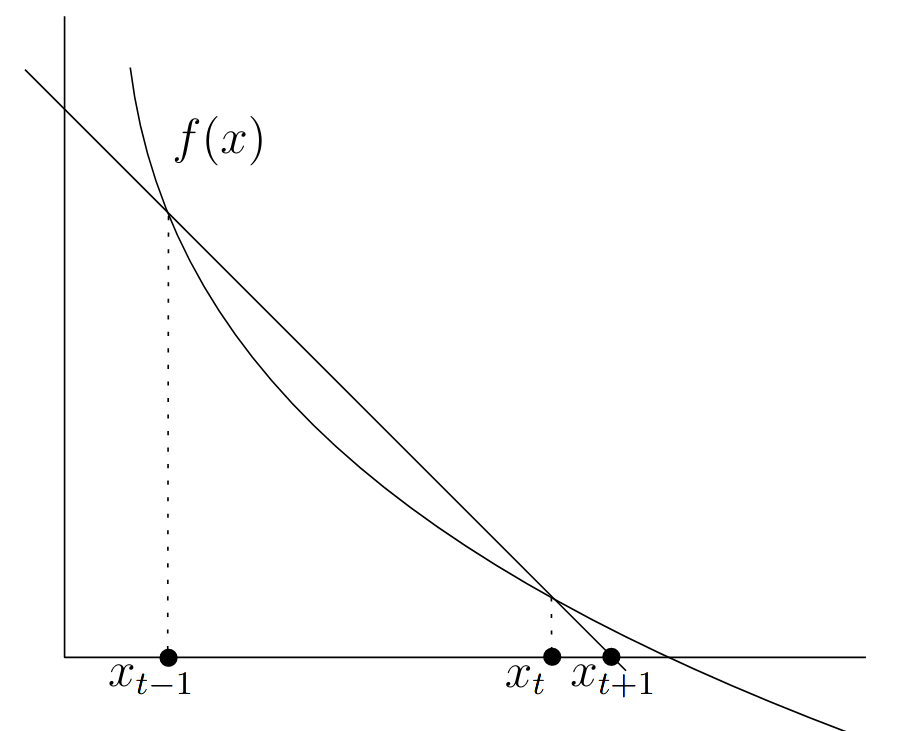
\includegraphics[width=0.6\textwidth,keepaspectratio]{secant_method}
  \end{figure}
  Constructs the line through $(x_{k-1}, f(x_{k-1}))$ and $(x_k, f(x_k))$.
\end{frame}


\begin{frame}
  \frametitle{The secant method III}
  \begin{itemize}
    \item is a \emph{derivative-free} version of the Newton-Raphson method.
    \item \textcolor{blue}{For optimization}: Apply secant method to $f'$ to optimize $f$:
          \begin{equation}
            x_{k+1} = x_k - f'(x_k) \frac{x_k - x_{k-1}}{f'(x_k) - f'(x_{k-1})}.
          \end{equation}
    \item yields a \textcolor{blue}{second-derivative free} version of Newton's method.
  \end{itemize}

  \vspace{1cm}

  \onslide<2->{%
    \begin{center}
      \textit{What about higher dimensions? Can't divide vectors..}
    \end{center}
  }
\end{frame}


\begin{frame}
  \frametitle{The secant condition}
  In $1$-d:
  \begin{align}
    H_k &:= \frac{f'(x_k) - f'(x_{k-1})}{x_k - x_{k-1}} \approx f''(x_k) \\
    &\Leftrightarrow f'(x_k) - f'(x_{k-1}) = H_k (x_k - x_{k-1}),
  \end{align}
  the \textcolor{blue}{secant condition}.
  \begin{itemize}
    \item Newton's method: $x_{k+1} = x_k - {f''(x_k)}^{-1} f'(x_k)$
    \item Secant method: $x_{k+1} = x_k - {H_k}^{-1} f'(x_k)$
  \end{itemize}
\end{frame}


\begin{frame}
  \frametitle{Quasi-Newton methods}

  \begin{equation}
    \nabla f(x_k) - \nabla f(x_{k-1}) = H_k (x_k - x_{k-1}) \approx \nabla^2 f(x_k) (x_k - x_{k-1})
  \end{equation}
  We therefore hope that $H_k \approx \nabla^2 f(x_k)$.

  \begin{equation}
    \text{Secant Method:} \quad x_{k+1} = x_k - H_k^{-1} \nabla f(x_k)
  \end{equation}

  \begin{itemize}
    \item $d=1$: unique number $H_k$ satisfying the secant condition
    \item $d>0$: secant condition $\nabla f(x_k) - \nabla f(x_{k-1}) = H_k (x_k - x_{k-1})$ has \textbf{infinitely} many \textit{symmetric} solutions
  \end{itemize}

  \begin{block}{}
    \textit{Any scheme of choosing in each step of the secant method a symmetric $H_k$ that satisfies the secant condition defines a \textcolor{blue}{Quasi-Newton method}.}
  \end{block}


\end{frame}

\begin{frame}
  \frametitle{Quasi-Newton methods II}

  \begin{itemize}
    \item Newton’s method is a Quasi-Newton method $\Leftrightarrow$
          $f$ is a nondegenerate \textbf{quadratic} function.
    \item $\Rightarrow$ Quasi-Newton methods \textit{do not generalize} Newton’s method but form a
          family of \textit{related} algorithms.
    \item First Quasi-Newton method by William Davidon in 1956
    \item But the paper got rejected for lacking a convergence analysis,
    \item was finally officially published in 1991
    \item \textcolor{blue}{methods of choice} in a number of relevant machine learning applications
  \end{itemize}

\end{frame}

\begin{frame}
  \frametitle{Developing a Quasi-Newton method}
  \begin{itemize}
    \item want to avoid matrix inversion
          $\Rightarrow$ directly deal with the inverse $H_k^{-1}$
    \item \textcolor{blue}{Given:} iterates $x_{k-1}, x_k$ and matrix $H_{k-1}^{-1}$
    \item \textcolor{blue}{Seeking:} next matrix $H_k^{-1}$ needed in next Quasi-Newton step
          \begin{equation}
            x_{k+1} = x_k - H_k^{-1} \nabla f(x_k)
          \end{equation}
    \item How to choose $H_k^{-1}$?
    \item Newton’s method: $\nabla^2 f(x_k)$ fluctuates only very little in the region of very fast convergence.
    \item Makes sense to have $H_k \approx H_{k-1}$ or $H_k^{-1} \approx H_{k-1}^{-1}$
  \end{itemize}
\end{frame}


\begin{frame}
  \frametitle{Greenstadt's family of Quasi-Newton methods}
  Greenstadt [Gre70]: Update
  \begin{equation}
    H_k^{-1} = H_{k-1}^{-1} + E_k,
  \end{equation}
  with $E_k$ an error matrix.
  \begin{itemize}
    \item Try to \textcolor{blue}{minimize error} subject to $H_k$ satisfying the \textbf{secant condition}!
  \end{itemize}

  Simple error measure: Frobenius norm
  \begin{equation}
    \Vert E \Vert_F^2 := \sum_{i=1}^{d} \sum_{j=1}^{d} E_{ij}^2
  \end{equation}
\end{frame}


\begin{frame}
  \frametitle{BFGS method}
  \begin{itemize}
    \item special version of Greenstadt
    \item is named after Broyden, Fletcher, Goldfarb and Shanno
          who all came up with it independently around 1970. Greenstadt mostly forgotten.
    \item Newton’s method needs to compute and invert Hessians\\
          $\Rightarrow$ cost of $\mathcal{O}(d^3)$ per iteration
    \item Any method in Greenstadt's family avoids computation of Hessian.
          \textbf{Only gradients are needed}.
    \item In the BFGS method, the cost per iteration drops to $\mathcal{O}(d^2)$.
    \item even this can be prohibitive $\rightarrow$ \textbf{limited memory BFGS}
    \item uses observation that we do not need $H_{k}^{-1}$, only $H_{k}^{-1} \nabla f(x_k)$
  \end{itemize}

\end{frame}
\end{document}
